
\subsection{Dataset}

Animals with Attributes (AwA2) data-set\footnote{\texttt{https://cvml.ist.ac.at/AwA2/}}~\cite{xian2018zero} consists of 37322 images of 50 animal classes with pre-extracted deep learning features for each image. We will use this data-set to explore different distance metrics. Throughout this project, we will be using KNN (implemented in \texttt{sklearn.neighbors.KNeighborsClassifier}) to perform classification tasks on the data-set.

\begin{table}[htbp]
\centering
\caption{Cross Validation Accuracy of KNN on Raw Data under Different Settings of $K$ }
\label{tab:cross-val}
\begin{tabular}{@{}ccccccc@{}}
\toprule
$K$    & Fold 1  & Fold 2  & Fold 3  & Fold 4  & Fold 5  & Avg Accuracy \\ \midrule
1   & 87.83\% & 87.27\% & 88.26\% & 87.87\% & 88.25\% & 87.90\%      \\
2   & 86.31\% & 85.38\% & 86.74\% & 86.00\% & 86.20\% & 86.13\%      \\
3   & 88.75\% & 87.81\% & 88.84\% & 87.78\% & 88.41\% & 88.32\%      \\
4   & 88.79\% & 87.83\% & 89.37\% & 88.23\% & 88.43\% & 88.53\%      \\
5   & 89.15\% & 88.43\% & 89.86\% & 88.72\% & 88.92\% & 89.02\%      \\
6   & 88.99\% & 88.35\% & 89.64\% & 88.88\% & 88.83\% & 88.94\%      \\
7   & 89.04\% & 88.79\% & 89.91\% & 88.77\% & 88.74\% & \textbf{89.05\%}      \\
8   & 89.04\% & 88.59\% & 89.82\% & 88.34\% & 88.37\% & 88.83\%      \\
9   & 88.99\% & 88.50\% & 89.57\% & 88.63\% & 88.57\% & 88.85\%      \\
10   & 88.84\% & 88.32\% & 89.33\% & 88.52\% & 88.37\% & 88.68\%      \\\bottomrule
\end{tabular}
\end{table}

To ensure the consistency in different experiments, we split the images in each category into 60\% for training and 40\% for testing. Throughout all experiments, the same training set will be used and accuracy results will be obtained from the testing set.

To begin with, we use K-fold cross-validation within the training set to determine the hyper-parameter $K$ for KNN model. The training set is split into 5 folds and the distance used is Euclidean distance. The cross-validation results of $K$ ranging from 1 to 10 are displayed in Table \ref{tab:cross-val}. We visualize the average score of $K$ ranging from 1 to 30 in Figure \ref{fig:cvk}. We can get optimal accuracy when $K$ equals 7, and when $K$ goes larger than 7, the accuracy shows a downward trend.

\begin{figure}
    \centering
    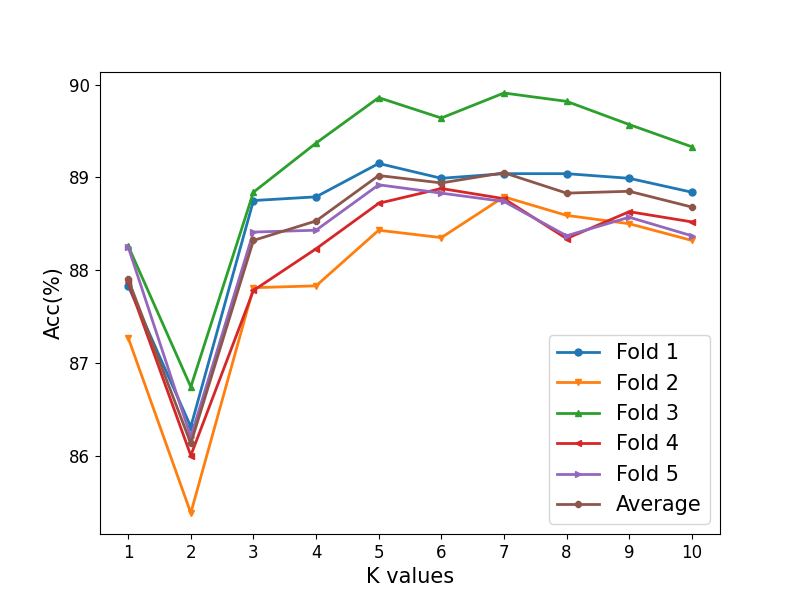
\includegraphics[width=0.6\textwidth]{img/KNN_res.png}
    \caption{Cross Validation Accuracy over $K$}
    \label{fig:cvk}
\end{figure}


\subsection{Experiment setting}

As different distance metrics may get different optimal $K$ value, in the following experiments, we test on $K$ from 3 to 10, 15 and 20. For traditional metrics, the distance is calculated directly. For supervised metric learning methods, we make use of the original labels to train the distance metric. 

For weakly-supervised metric learning methods, since they require pairs/groups of similar/dissimilar data points,
we will sample similar and dissimilar points from the labeled data-set. To be specific, for pairs learners, pairs (tuple of two points from the data-set), and pair labels (integer indicating whether the two points are similar (+1) or dissimilar (-1)), are sampled randomly from the original data-set with category labels. To sample positive pairs (of label +1), the method will look at all the samples from the same label and sample randomly a pair among them. To sample negative pairs (of label -1), the method will look at all the samples from a different class and sample randomly a pair among them.